\documentclass[11pt]{report}
\usepackage{graphicx}
\graphicspath{{../Images/}}
\newcommand{\bsat}{b_{\mathrm{sat}}}
\newcommand{\qsat}{Q_{\mathrm{sat}}}
\newcommand{\xsat}{x_{\mathrm{sat}}}
\newcommand{\xunsat}{x_{\mathrm{unsat}}}
\newcommand{\xch}{x_{\mathrm{Chol}}}
\newcommand{\nbound}{b_{\mathrm{tot}}}
\newcommand{\lo}{l_{\mathrm{o}}}
\newcommand{\ldo}{l_{\mathrm{do}}}
\newcommand{\m}[2]{M_{\mathrm{{#1},{#2}}}}
\newcommand{\mself}[1]{M_{\mathrm{#1}}}
\newcommand{\nachr}{nAChR}
\title{SUPPLEMENTARY MATERIAL: Boundary lipids of the nicotinic acetylcholine receptor: spontaneous partitioning via coarse-grained molecular dynamics simulation}
\author{Liam Sharp, Reza Salari, and Grace Brannigan}
\begin{document}
%\maketitle
\begin{center}
\Large 	
{ \bf SUPPLEMENTARY MATERIAL} 

Boundary lipids of the nicotinic acetylcholine receptor: spontaneous partitioning via coarse-grained molecular dynamics simulation

{Liam Sharp, Reza Salari, and Grace Brannigan}

\end{center}
\normalsize
		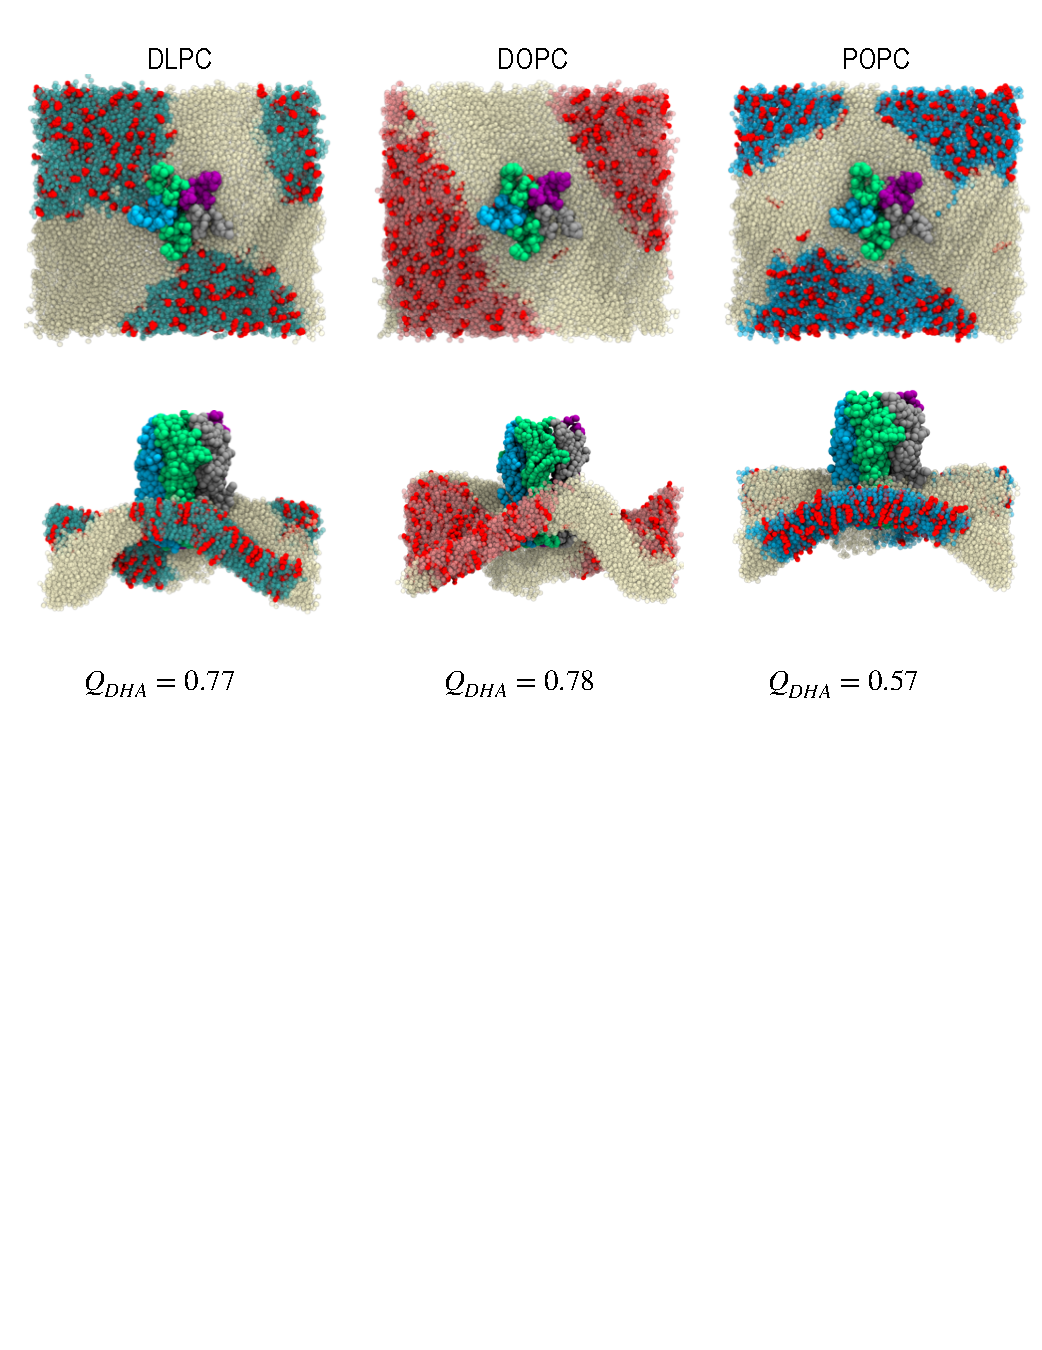
\includegraphics[width=1\linewidth]{SI_Chains.pdf}
	
		{\bf Figure S1}. {Membrane domain formation and protein domain partitioning in small membranes.} Two viewpoints are shown of the final frame of a single nAChR in a membrane composed of dDHA-PE:$X$:CHOL 42.5:42.5:15, where $X$ is either DLPC, DOPC, or POPC. Subunits are colored: $\alpha$: green, $\beta$: purple, $\delta$: gray, $\gamma$: cyan. Lipids are colored: Chol: red, dDHA-PE: white, DLPC: teal, DOPC : pink, POPC : cyan. Large deformations and undulations are caused by the highly flexible domains formed by dDHA-PE and the conical shape of nAChR.  %POPC, the only hybrid lipid used in these simulations, unexpectedly, comprises a greater fraction of the boundary region than DLPC or DOPC.
	

\clearpage
		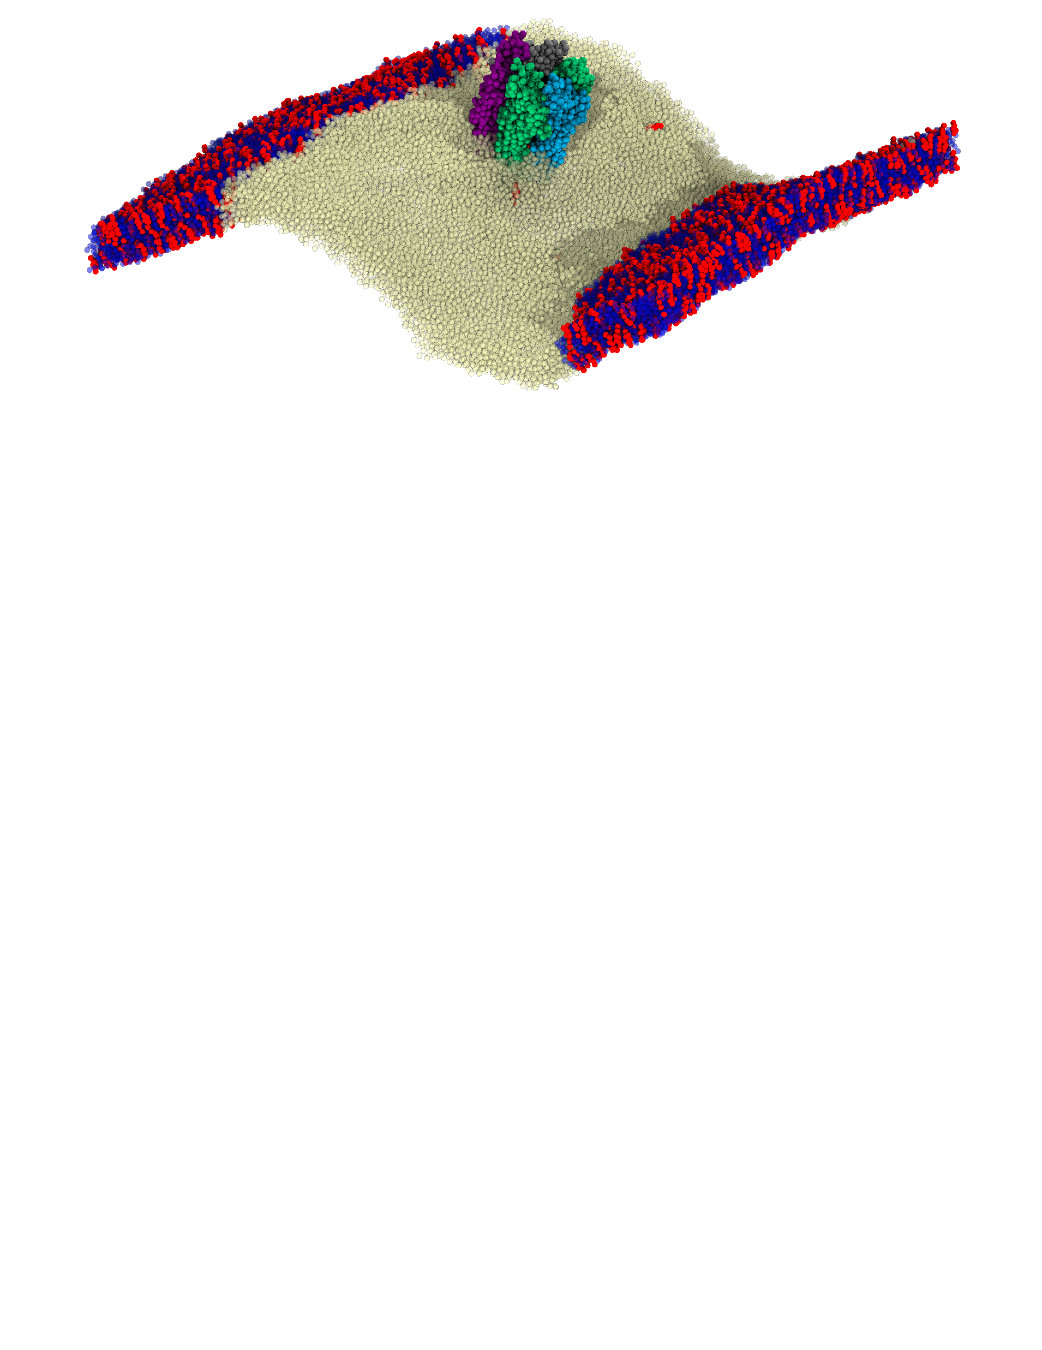
\includegraphics[width=1\linewidth]{Memb_Curve.pdf}
		{\bf Figure S2. }Alternate view of membrane from Figure 3A. The $\ldo$ domain formed by dDHA-PE (white) is highly flexible with large undulations; this flexibility may also result in more favorable incorporation of the cone-shaped \nachr~transmembrane domain. 

\end{document}
	